
\chapter{Marine bacterial, archaeal and eukaryotic diversity and community structure on the continental shelf of the Western Antarctic Peninsula}\label{ch:mirada}

\chapterdisclaimer{This chapter is adapted from the following publication: \\
Luria, C. L., Ducklow, H. W., and Amaral-Zettler, L. A. (2014). Changes in bacterial, archaeal and eukaryotic community structure in along a hypothesized climatic gradient in the western Antarctic Peninsula. \emph{Aquatic Microbial Ecology} 73, 107-121.\\
\\
Linda Amaral-Zettler and Hugh Ducklow designed and conducted the study. Linda Amaral-Zettler contributed sequence data. Catherine Luria and Linda Amaral-Zettler performed data analyses. Catherine Luria wrote the manuscript with guidance and input from Linda Amaral-Zettler and Hugh Ducklow. 
}

\section{Abstract}\label{sc:abstract}

The classic view of polar ocean foodwebs emphasizes large predators sustained by energy and materials flow through short, efficient diatom-krill-predator food chains. Bacterial activity is generally low in cold polar waters compared to lower latitudes. This view appears to be changing, with new studies of microbial foodwebs in Arctic and Antarctic oceans. We characterized bacterial, archaeal, and eukaryotic community diversity and composition from two depths (near surface and below the euphotic zone) at four sites, including the inshore and offshore, and north and south corners of a sampling grid along the western coast of the Antarctic Peninsula (WAP). We detected up to 2-fold higher richness in microbial eukaryotes at surface and deep inshore northern stations as compared to southern ones but offshore northern and southern stations revealed either no trend or higher richness at depth in the south. In contrast, bacterial and archaeal richness showed no significant differences either inshore or offshore at northern versus southern extents but did vary with depth. Archaea were virtually absent in summer surface waters but were present in summer deep and winter surface samples. Overall, winter bacterial and archaeal assemblages most closely resembled summer sub-euphotic zone assemblages, reflecting well-established seasonal patterns of water column turnover and stratification that result in an isolated layer of ``winter water'' below the euphotic zone. Inter-domain heterotroph-phototroph interactions were evident from network analysis. The WAP is among the most rapidly warming regions on earth. Our results provide a baseline against which future change in microbial communities may be assessed.

\section{Introduction}\label{sc:introduction}

Microbes are the most abundant organisms in the biosphere and their activities determine many biogeochemical properties of marine ecosystems \citep{Azam1983-wo, pwah07}. Characterizing microbes in the environment has historically proven difficult due to their small size and vast diversity, but recent advances in sequencing technology have allowed for great advances in efforts to describe microbial community structure and function \citep{dk05,smhwhnah06,fstcscd08, Yooseph:2010aa}. Evidence is mounting that microbial community composition is sensitive to environmental variability. For example, recent findings demonstrate that water mass physical and chemical, as well as biological properties drive microbial community structure \citep{alnsh11}. However, basic information on microbial community structure is still scarce for many areas of the global ocean.

Our study was part of the Microbial Inventory Research Across Diverse Aquatic Long Term Ecological Research Sites (MIRADA-LTERS) Project (\url{http://amarallab.mbl.edu}). The LTER Network of 25 aquatic and terrestrial, and marine and freshwater sites is a rich resource for comparative study of microbial communities and the processes they catalyze \citep{rcfbdgghmmsww12, arm13}. The Palmer Antarctica LTER study region is a pelagic marine ecosystem, with ongoing research examining the impacts of seasonal to inter-annual climate variation on sea ice, plankton food webs and ecosystem biogeochemistry \citep{dcddghmmmms12}. Our study region extends \textasciitilde{} \SI{200}{\km} from the coast to the open ocean and \textasciitilde{} \SI{400}{\km} from north to south and encompasses several sub-regions, each with its own combination of potential forcing factors on microbial communities \citep{dsvse12}.

Like other high latitude areas, the WAP experiences extreme seasonal variations, ranging from near total darkness, deep vertical mixing, extensive sea ice cover and minimal photosynthetic organic matter formation in winter, to the opposite conditions in summer. Bacterial abundance and productivity increase from winter to summer as primary production increases and the water warms from the freezing point (-1.8\textdegree C) to about 0 to +2\textdegree C \citep{dsvse12}. Bacterial diversity is high in cold, dark, low productivity waters in winter, and much lower in summer \citep{mg07,grwddecm12}. In summer (January) 2008, we sampled the four corners of the Palmer LTER study grid (Figure \ref{fig:ltergrid}) in order to contrast highly productive inshore sites with less productive offshore sites and to compare northern and southern sites differing in the annual extent and duration of sea ice cover.

\begin{figure}[ht!] 
\centering 
	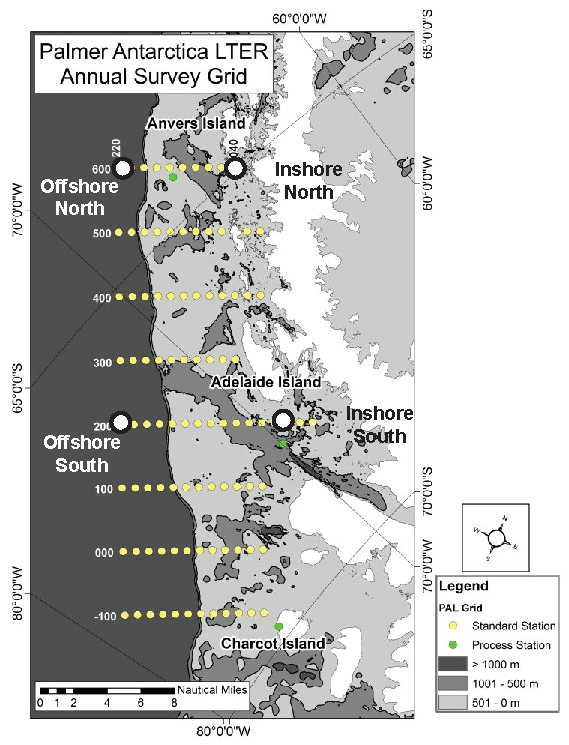
\includegraphics{Chapter_2_MIRADA/Figures/Figure_1_Map} 
	\caption[Map of the Palmer LTER study region.]{Palmer LTER study region along the western Antarctic Peninsula. The white circles indicate the sampling sites.~Land is shown in white, shades of gray indicate depth of water offshore according to legend, and numbers along the sampling grid correspond to LTER designated sampling names.} 
	\label{fig:ltergrid} 
\end{figure}

We sampled and described all three domains of microbial life---Eukarya, Bacteria, and Archaea---through small subunit (SSU) rRNA gene hypervariable amplicon sequencing in order to investigate spatio-temporal variation within domains and the linkages between microbial trophic levels. We found evidence of vertical stratification and temporal variation in community structure corresponding to the seasonal evolution of the upper water column. There were few differences between northern and southern sites. Significant variation between northern and southern assemblages was only evident for microbial eukaryotes and not their bacterial and archaeal counterparts. These results provide core data for comparative study with other aquatic systems, and furnish a baseline against which future changes may be assessed on a range of time and space scales.

\section{Materials and Methods}\label{sc:materials-and-methods}

\subsection{Sample Collection and Processing}\label{ssc:sample-collection-and-processing}

Sampling was conducted on the annual Palmer LTER midsummer research cruise (January -- February 2008). We drew samples from \SI{10}{\m} and \SI{100}{\m} depths from the northern and southern, inshore and offshore corners of the Palmer LTER sampling grid that lies along the western coast of the Antarctic Peninsula (Figure \ref{fig:ltergrid}). We collected duplicate samples using a rosette equipped with 10-liter Niskin bottles and Conductivity, Temperature and Depth (CTD) sensors. To contrast summer and winter water, we also collected an additional Austral winter sample from \SI{10}{\m} depth at the northern, inshore sampling site in August 2008 using a submersible pump with silicone tubing. Environmental data, including nitrate (\ce{NO3}), phosphate (\ce{PO4}), silicate (\ce{SiO4}), particulate nitrogen (P\ce{N}), total nitrogen (T\ce{N}), particulate organic carbon (PO\ce{C}), dissolved organic carbon (DO\ce{C}), chlorophyll \textit{a} (chl \textit{a}), \ce{14C}-primary production, and bacterial abundance and production, were collected through the Palmer Station LTER (\url{http://oceaninformatics.ucsd.edu/datazoo/data/pallter/datasets}). Protocols for these measurements are available in the metadata for each environmental variable. Limited environmental data were available for the winter sample.

We filtered water samples (\SIrange{1}{2}{\L}) through \SI{0.2}{\micro\m} Sterivex\texttrademark~ cartridges (Millipore, Billerica, MA), preserved genomic DNA by flooding the 2-ml filter cartridge reservoir with sucrose lysis buffer (40 mM EDTA, 50 mM \ce{Tris-HCl}, 0.75 M sucrose), and stored the filters at -80\textdegree C until processing. We extracted DNA using a Puregene DNA extraction kit (Qiagen, Valencia, CA) with modifications as described in \citet{amdh09} and stored the DNA at -20\textdegree C until PCR amplification. Bacterial and archaeal V6 16S rRNA and eukaryotic V9 18S rRNA gene hypervariable regions were amplified as described previously \citep{hwmhnbs07, amdh09}, using ``barcoded'' primers which allowed for multiplexed sequencing (see \url{http://vamps.mbl.edu/resources/primers.php} for details). For each sample, we pooled triplicate \SI{50}{\micro\l} PCR reaction products to minimize propagation of PCR errors and purified them using a QIAquick column-based purification kit (Qiagen, Valencia, CA). We sequenced purified amplicons on a 454 Genome Sequencer FLX (Roche, Basel, Switzerland) according to the manufacturer's protocols using the LR70 kit. We trimmed and filtered raw sequence reads as previously described \citep{hhmsw07}. Briefly, 5 bp barcodes were detected and removed, if exact matches to the barcode were not recovered these reads were discarded. Further quality filtering was achieved by requiring exact matches to the proximal and distal primers, removal of any N's in the sequence reads, and removal of all reads less than 50 nucleotides in length. We assigned Operational Taxonomic Units (OTUs) at a 3\% (Bacteria and Archaea) or 6\% (Eukarya) sequence identity clustering level (SLP-PWAL; \citet{hwms10}). We chose a more conservative cut-off for eukaryotic clustering to accommodate microheterogeneities existing in many eukaryotic taxa. In many cases, we were able to achieve genus-level identifications with this cluster width. We also removed all metazoan OTUs from downstream analyses.

\subsection{Alpha and Beta Diversity Estimation}\label{ssc:alpha-and-beta-diversity-estimation}

We determined parametric modeling-based estimates of species richness for Bacteria and Archaea using the CatchAll program \citep{bunge2012estimating} and estimated eukaryotic richness using the non-parametric Chao2 estimator in SPADE \citep{cs10}. For multivariate methods, we employed bacterial and archaeal abundance matrices while eukaryotic abundances were converted to incidence-based (presence/absence) matrices. PC-ORD \citep{p10} was used to conduct a two-way cluster analysis for the archaeal dataset. We generated Morisita-Horn similarity indices for Bacteria and Archaea in EstimateS \citep{c09} and employed Jaccard similarity indices for eukaryotic data in Primer-E (v6, Plymouth, UK). Bray-Curtis and Morisita-Horn similarity indices were generated for resampled bacterial and archaeal data sets. SIMPROF (Primer-E) analyses allowed us to test for significant differences between biological replicates while ANOSIM allowed us to test for differences between samples. We visualized the results using non-metric multidimensional scaling (NMDS) (Primer-E). We performed all calculations using complete abundance matrices, as well as resampled matrices in which the number of sequences reads per sample was made equal through random resampling: 1219 sequences per sample for Bacteria (3218 with replicates pooled), 1005 for Archaea (2502 with replicates pooled), 2370 for Eukarya (4911 with replicates pooled). We only showed resampled data results where resampling deviated from the full dataset result.

\subsection{Unimodal Multivariate Analysis}\label{ssc:unimodal-multivariate-analysis}

We employed CANOCO 4.5 (Microcomputer Power, Ithaca, NY) \citep{Ter-Braak:2002aa} to relate our OTUs to environmental properties. Environmental data were transformed using $ln(x + 0.1)$ and temperature was adjusted to remove negative values by adding 1\textdegree C to each value. Preliminary Detrended Correspondence Analysis yielded gradients close to three so we chose to continue our analyses using the CCA unimodal approach. We employed the automatic forward selection feature in CANOCO to ensure selection of parameters that have low cross-correlation and explain the most variance. The significance of the first CCA axis and all CCA axes combined was tested using Monte Carlo permutation tests with 499 permutations \citep{Ter-Braak:2002aa}.

\subsection{Network Analysis and Data Visualizations}\label{ssc:network-analysis-and-data-visualizations}

We examined co-occurrence patterns across domains using network analysis and significant linear Pearson correlations. For the input matrices we removed all singleton OTUs and only considered OTUs that occurred in at least 50 percent of the samples. We used Cytoscape \citep{smobwr} to visualize the resulting data and only considered significant correlations with an R-value \textgreater{}0.9. We generated bacterial taxonomic bar graphs using Global Alignment Sequence Taxonomy (GAST) \citep{hdhwrs08} and used Qiime v1.4.0 \citep{Caporaso2010-ee} to graphically display the output. The R package routines gplots and heatmap.2 were used to generate the heatmap summary of all microbial eukaryotic OTUs that were encountered with a frequency of greater than 1\% in a given site \citep{t08}. All of our sequence data are MIMARKS-compliant \citep{Yilmaz:2011aa} and have been deposited in the National Center for Biotechnology Information normal and Sequence Read Archives under the accession number SRP041427. Bacterial V6 data were previously deposited under SRP016030 while Eukaryotic V9 were previously deposited under SRP000903. Copies of the MIMARKS table and chapter figures can be accessed at: \url{https://github.com/cmluria/dissertation/Chapter_2_MIRADA}. 

\section{Results}\label{sc:results}

\subsection{Sampling site characteristics}\label{ssc:sampling-site-characteristics}

\afterpage{
\clearpage
\begin{landscape}
\begin{table}
\centering
\caption[Contextual data for sites sampled.]{Contextual data for sites sampled. Differences between depths, inshore and offshore, and north and south comparisons between samples were assessed using student’s t-tests.}
\label{ch1:tab1}
\small
\begin{tabular}{@{}lllllll@{}}
\toprule
Variable                                                     & 10-m Overall & 100-m Overall & 10-m Inshore & 10-m Offshore & 10-m North & 10-m South\\ \midrule
Density                                                      & 27.2**            & 27.4**             & 27.2              & 27.2               & 27.2**          & 27.1**          \\
Salinity                                                     & 33.8**            & 34.2**             & 33.8              & 33.9               & 33.8            & 33.8            \\
Oxygen (µmol/l)                                              & 357*              & 276*               & 366               & 348                & 362             & 352             \\
Temperature (°C)                                             & 0.756             & -0.224             & 0.773             & 0.739              & 0.765           & 0.747           \\
NO3 (µmol/l)                                                 & 18.6*             & 24.8*              & 16.5*             & 20.8*              & 19.5            & 17.8            \\
NO2 (µmol/l)                                                 & 0.38              & 0.28               & 0.25              & 0.5                & 0.35            & 0.4             \\
PON (µmol/l)                                                 & 47.6              & ND                 & 79.9              & 15.2               & 69.2            & 25.9            \\
Total N (µmol/l)                                             & 28.3**            & 36.3**             & 25.1*             & 31.4*              & 29.4            & 27.2            \\
PO4 (µmol/l)                                                 & 1.58***           & 2.10***            & 1.50*             & 1.65*              & 1.6             & 1.55            \\
Si (µmol/l)                                                  & 53.2              & 68.6               & 70.8**            & 35.5**             & 53.2            & 53.2            \\
DOC (µmol/l)                                                 & 45.7              & 43.4               & 46.4              & 45                 & 46.5            & 45.7            \\
POC (µmol/l)                                                 & 210               & ND                 & 349               & 71.8               & 306             & 115             \\
Chlorophyll \emph{a} (µg/l)                                         & 1.71              & 0.147              & 3.21*             & 0.215*             & 2.13            & 1.3             \\
Fluorescence (mg/m$^3$)                                         & 2.3               & 0.189              & 4.1               & 0.506              & 3.14            & 1.47            \\
Bacterial dens. ($10^6$/ml)                                  & 0.227             & 0.225              & 0.242             & 0.212              & 0.189*          & 0.266*          \\
Leucine inc. (pmol/l)                               & 14.6              & ND                 & 22.9              & 6.37               & 18.8            & 10.5            \\ \midrule
                                                             &                   &                    &                   &                    &                 &                 \\
\multicolumn{7}{l}{* $p < 0.1$, ** $p < 0.05$, *** $p < 0.01$}  
\end{tabular}
\end{table}
\end{landscape}
}

The waters in the WAP were consistently cold (<1\textdegree C) and experienced dramatic fluctuations in day length and sea ice cover during the study period. In the austral summer, deep samples (100-m) were more saline and had higher nutrient concentrations (\ce{PO4}, \ce{NO3}, TN, \ce{SiO4}), while surface samples (10-m) contained higher phytoplankton biomass (chl \textit{a}; Table \ref{ch1:tab1}). Within surface samples, we observed differences between inshore and offshore sites, with greater bacterial production and organic substrates (POC and PON) at inshore sites (Table \ref{ch1:tab1}). In general there were not significant environmental differences between the corresponding northern and southern sampling stations (Table \ref{ch1:tab1}).


\subsection{Microbial Community Structure}\label{ssc:microbial-community-structure}

Our three-domain assessment of the microbial communities of the WAP pelagic ecosystem generated \textgreater{}150,000 bacterial, \textgreater{}50,000 archaeal, and \textgreater{}60,000 eukaryotic rRNA amplicon reads from the Palmer LTER study region along the WAP. We selected these sites in order to examine how microbial communities vary with depth, distance from shore, and latitudinal differences in sea ice cover.

\begin{figure}
	[htbp] \centering 
	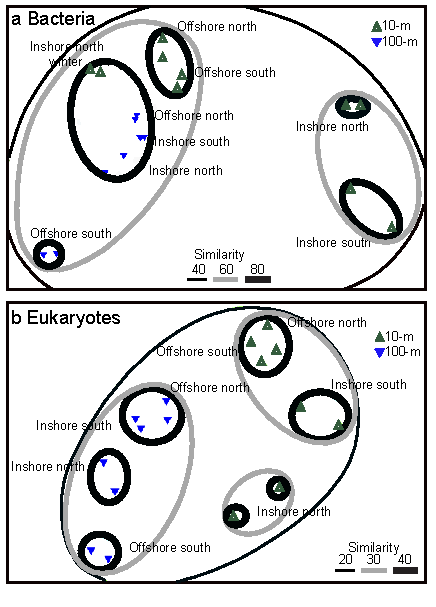
\includegraphics{Chapter_2_MIRADA/Figures/Figure_2_MDS_new_2012_75mm_BW_2013} 
	\caption[Non-metric multidimensional scaling of bacterial Morisita-Horn and eukaryotic Jaccard similarity matrices.]{Non-metric multidimensional scaling of (a) bacterial Morisita-Horn and (b) eukaryotic Jaccard similarity matrices. Bacterial ordination based on samples collected in January and August 2008. Eukaryotic (minus metazoan OTUs) ordination based on samples collected during January 2008 only.} 
	\label{fig:nmds1.1} 
\end{figure}

Bacterial community composition varied significantly by depth (ANOSIM, $p = 0.007$ full, $p = 0.004$ resampled), and slightly among surface samples between inshore and offshore samples (ANOSIM, $p = 0.08$ full, $p = 0.06$ resampled), but showed no significant north-south differences in community structure. NMDS and hierarchical clustering revealed that the inshore surface communities fell into two groups with 60\% similarity, one composed solely of inshore surface samples and one containing all other samples including offshore surface, winter surface and all deep samples, also sharing 60\% similarity (Figure \ref{fig:nmds1.1}). All bacterial samples taken together were 40\% similar to each other. The winter surface sample was more similar to summer deep samples than to any summer surface sample from the same station (Figure \ref{fig:ch1:supp1}). SIMPER analysis showed that 7 OTUs, identified as \textit{Candidatus} Pelagibacter, Oceanospirallales, \textit{Balneatrix}, Flavobacteriaceae, SAR324, \textit{Roseobacter} and Phycisphaeraceae, accounted for over 33\% of the variation between surface and deep communities. Eukaryotes had the greatest degree of variation among samples with some samples having only 20\% similarity. Eukaryotic community composition varied significantly with depth and distance from shore (ANOSIM, $p = 0.001$ and 0.03 respectively for the full dataset; $p= 0.001$ and 0.027 for the resampled dataset), but as with bacterial communities failed to exhibit large differences in beta diversity (between sample diversity) between the north and south stations. Individual eukaryotic OTUs were unable to explain more than 0.5\% of this variation (SIMPER). We detected little variation among archaeal communities (summer 100-m and winter surface) due in part to our inability to detect archaea in surface summer samples and there were few differences in the structure of corresponding northern and southern communities (e.g., northern vs.~southern inshore samples) (Figure \ref{fig:cca1.1}). We did observe significantly higher eukaryotic alpha diversity (species richness) at the northern inshore site (Figure \ref{fig:richness1}) and differences in the relative recoveries of individual eukaryotic OTUs (Figure \ref{fig:ch1:supp2}).

\begin{figure}[htbp] 
\centering 
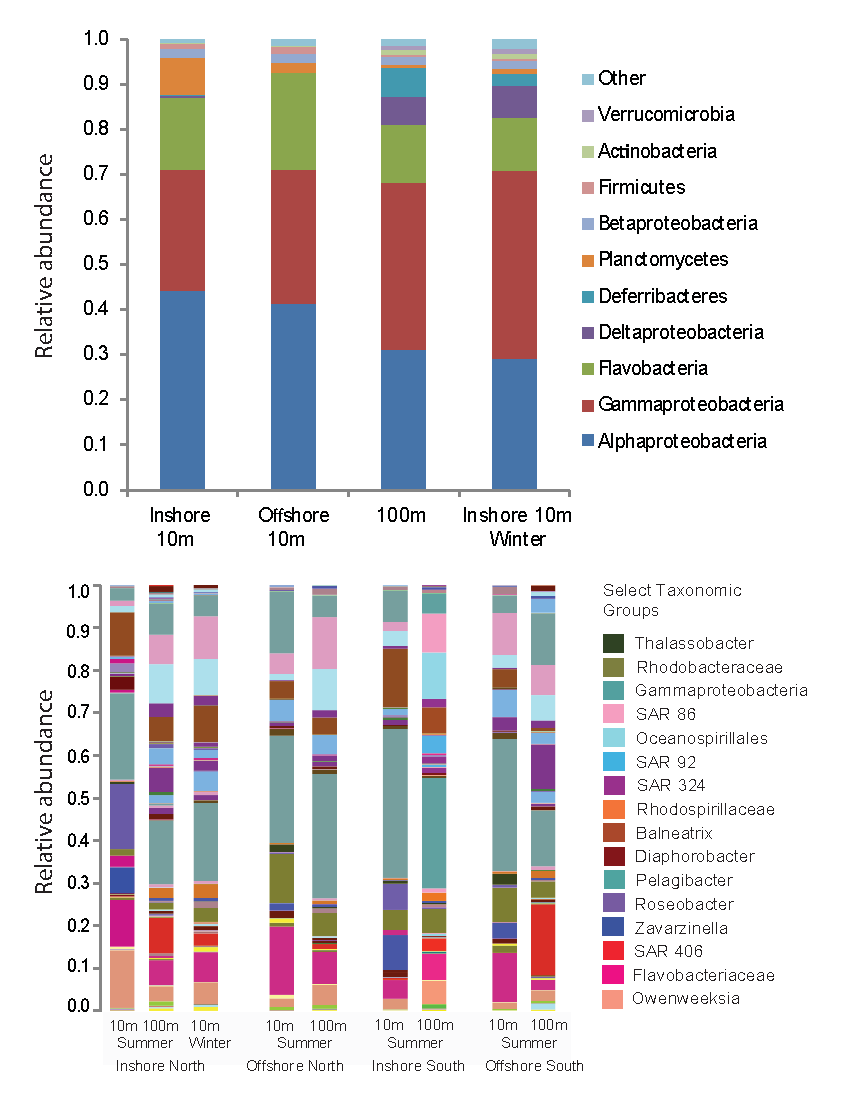
\includegraphics[width=1.0\textwidth]{Chapter_2_MIRADA/Figures/Supplemental_1_Qiime_taxonomic_summary} 
\caption[Relative abundance of most common bacterial taxa from different sets of sites.]{Relative abundance of most common bacterial taxa from (a) coarser taxonomic resolution for inshore and offshore 10 m (north and south pooled), 100 m (north and south inshore and offshore pooled), and winter inshore surface (north only) samples. (b) More fine scaled taxonomic resolution bar graphs for summer vs.~winter, inshore vs.~offshore, and North vs.~South.} 
\label{fig:ch1:supp1} 
\end{figure}


\begin{figure}
	[htbp] \centering 
	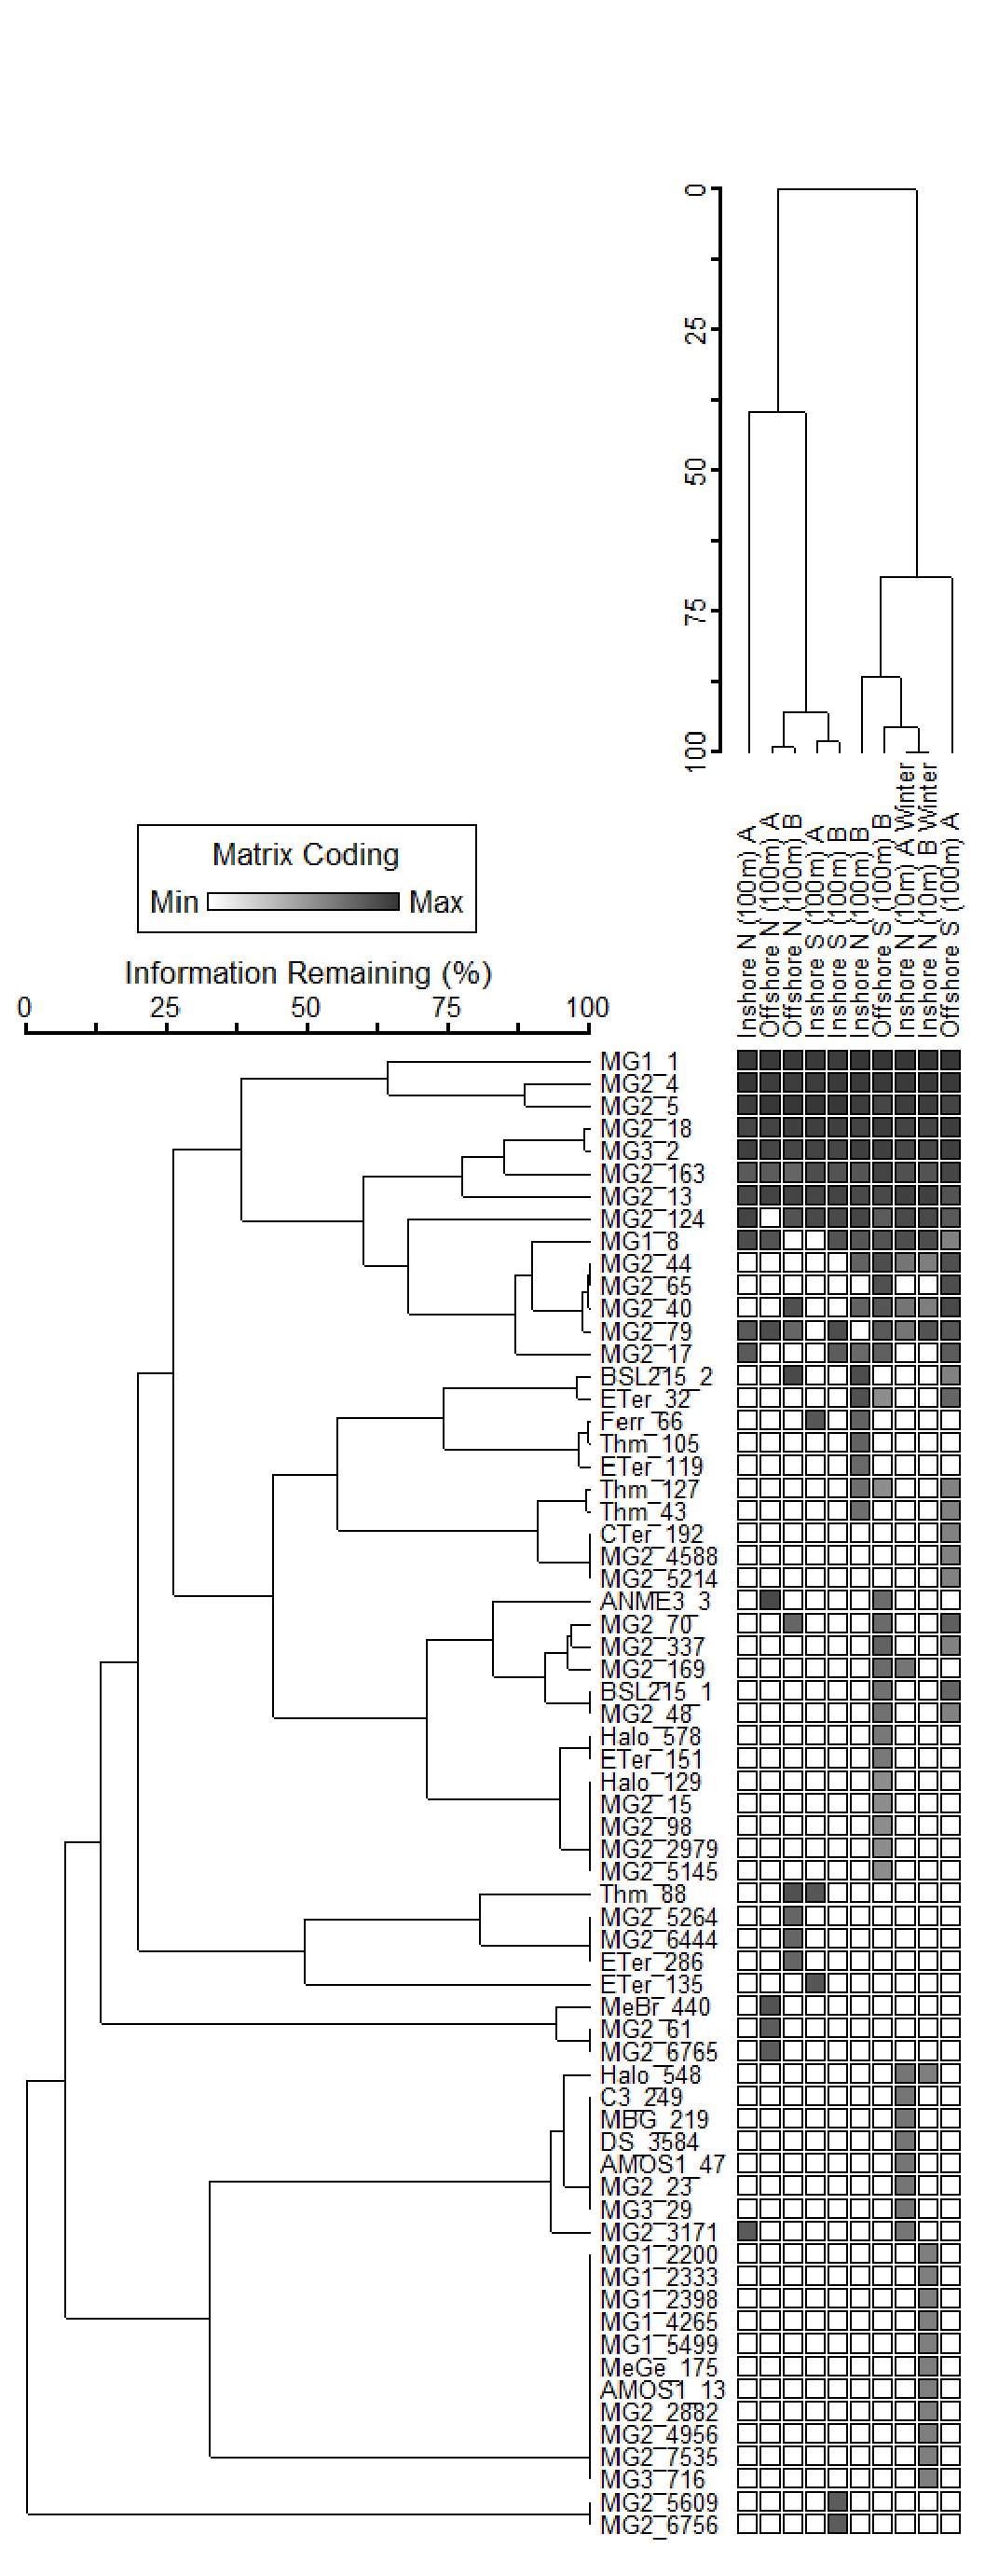
\includegraphics[width=0.5
	\textwidth]{Chapter_2_MIRADA/Figures/Figure_4_PAL_Av6_2way_notrans_Relmax_SOR_aveneigh} 
	\caption[Archaeal two-way cluster analysis.]{Archaeal two-way cluster analysis. Samples were collected from 100-m depth in January 2008 and from the surface in August 2008 (winter). Abbreviations are as follows: MG1 (Marine Group I Crenarchaeota; MG2 Marine Group II Euryarchaeaota; MG3 Marine Group III Euryarchaeota; remaining are miscellaneous Euryarchaeota groups). The matrix coding denotes the relative abundance within the matrix for a given OTU.} 
	\label{fig:cca1.1} 
\end{figure}

\begin{figure}
	[htbp] \centering 
	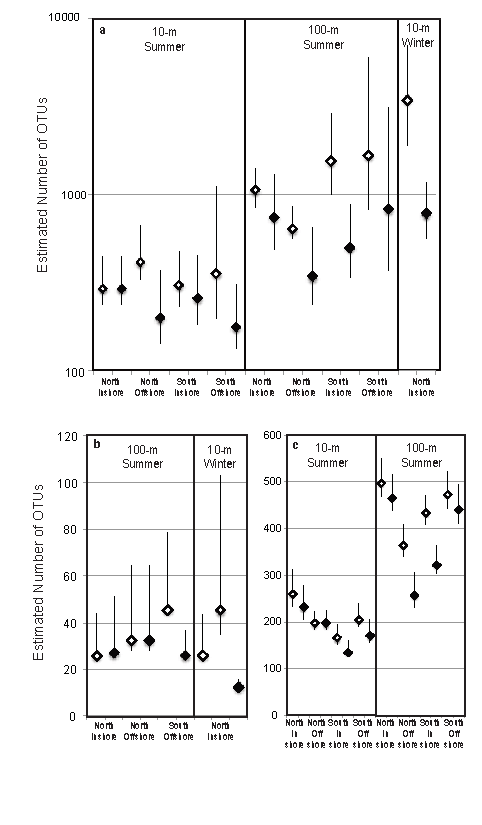
\includegraphics[width=0.7
	\textwidth]{Chapter_2_MIRADA/Figures/Figure_6_PAL_alpha_comp_75mm} 
	\caption[Estimated OTU richness for Bacteria, Archaea, and Eukarya at different sites.]{Species richness estimates of: (a) bacterial, (b) archaeal and (c) eukaryotic OTUs with Bonferroni-corrected 95\% confidence intervals for all samples across a given domain. Filled diamonds are for resampled data. For each of the bacterial samples two replicates were pooled. Eukaryotic diversity estimation required the two replicate samples to calculate a single incidence-based richness estimate for a given pair of samples. For archaeal estimates, south offshore 100-m and winter north inshore replicates are shown individually, north and south offshore 100-m replicates were pooled, and north offshore 100-m estimates were not done. Bacterial and archaeal estimates were calculated using CatchAll while eukaryotic estimates were calculated using Chao2 as implemented in SPADE.} \label{fig:richness1} 
\end{figure}

\begin{figure}[htbp] 
\centering 
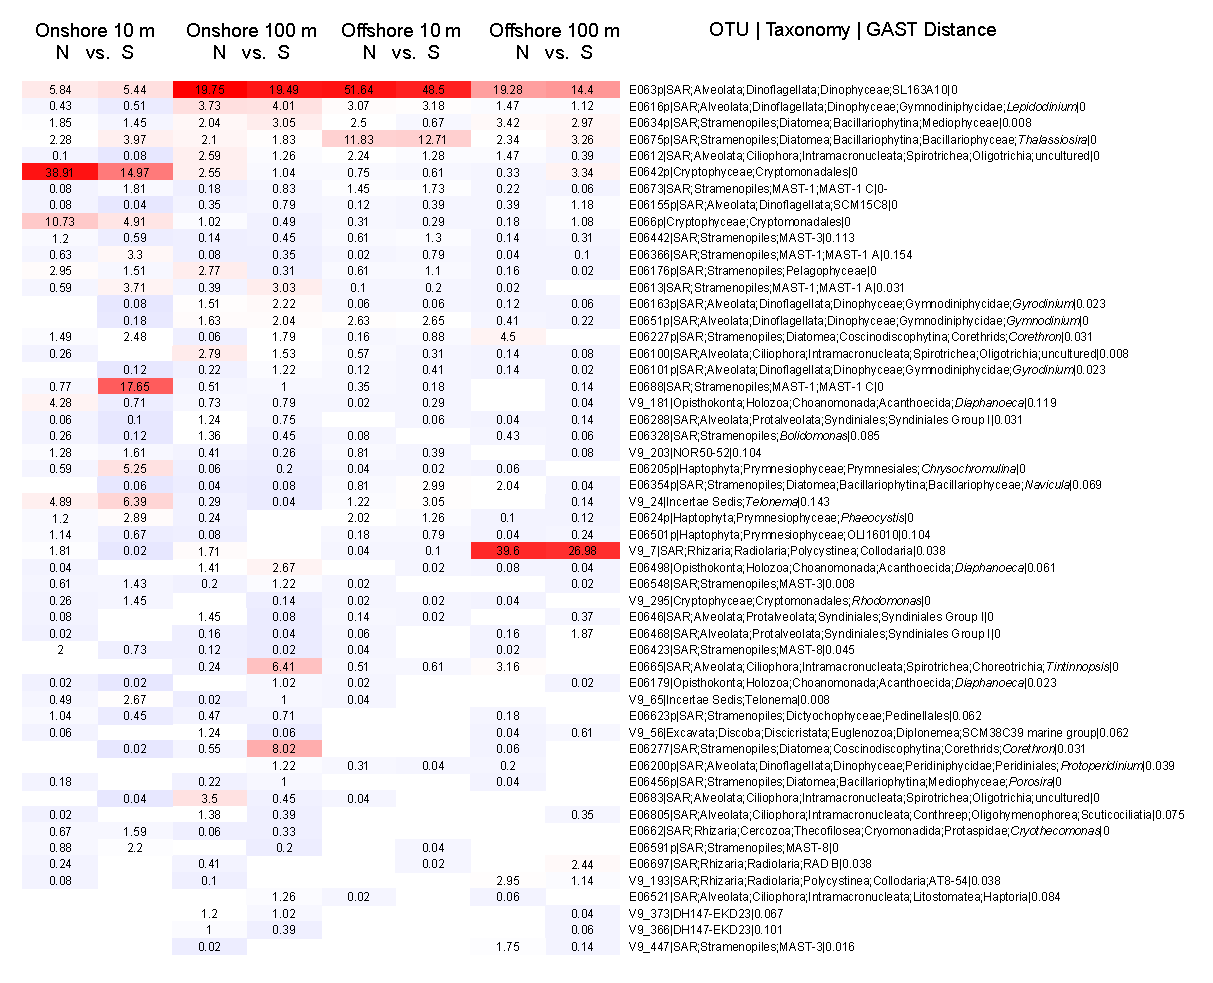
\includegraphics[width=\textwidth]{Chapter_2_MIRADA/Figures/Supplemental_2_euk_random_Rplot_4ms} 
\caption[Heatmap of eukaryotic OTUs.]{Heatmap of eukaryotic OTUs recovered at a frequency of more than 1\% at a given station. Hot colors indicate higher percentages while cooler colors indicate lower percentages, with actual values superimposed over colors. Data shown are normalized by randomly resampling data to the lowest sampling effort. The depth of taxonomic resolution available in the V9 region varied by taxon and is displayed to the right along with Global Alignment for Sequence Taxonomy \citep{hdhwrs08} distance values to the nearest relative in GenBank.} 
\label{fig:ch1:supp2} 
\end{figure}

\begin{figure}
	[htbp] \centering 
	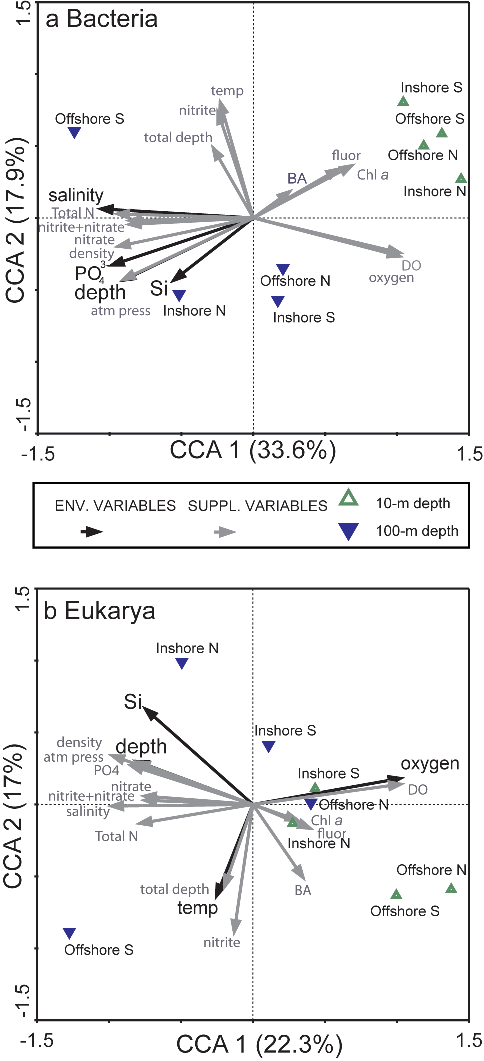
\includegraphics{Chapter_2_MIRADA/Figures/Figure_3_CCA} 
	\caption[Canonical correspondence analysis based on summer bacterial and eukaryotic OTU libraries.]{Canonical correspondence analysis based on (a) bacterial and (b) eukaryotic OTU libraries from water samples collected in January 2008. Explanatory variables (black arrows) and supplementary variables (grey lines) are shown.} 
	\label{fig:cca1.2} 
\end{figure}

We conducted further analyses to identify the linkages between community composition and environmental conditions. We were especially interested in co-occurrence patterns between bacteria and photosynthetic eukaryotes. CCA biplots summarized the relationships between environmental variables and bacteria and eukaryotes (Figure \ref{fig:cca1.2}). The underlying environmental variables determining community structure differed between bacterial and eukaryotic domains. For bacteria, CCA axis 1 was most closely correlated with salinity while CCA axis 2 was most closely correlated with silicate. The first CCA axis explained 33.6\% of the variance in the dataset and the first two axes combined explained 51.5\%. In addition to salinity and silicate, depth and phosphate were also significant explanatory variables shaping bacterial community structure. More so than NMDS, the bacterial CCA analysis showed a marked separation between shallow and deep samples along the vertical salinity gradient. As with NMDS, no obvious north-south separation between samples was evident in our biplots.


Eukaryotic CCA analysis showed a less marked difference between community structures at 100-m than for bacterial communities. The first CCA axis was defined by oxygen and the second by temperature and explained 22.3\% (Axis 1) and 39.3\% (Axes 1 \& 2) of the variation in the dataset respectively. The offshore south 100-m sample in particular was most positively correlated with higher temperature as was seen in the bacterial community analyses.

Due to the limited number of archaeal samples relative to environmental parameters available, we chose to conduct a two-way cluster analysis to explore the relationship between samples and OTU groups (Figure \ref{fig:cca1.1}) instead of conducting a CCA. The resulting two-way cluster diagram shows shared OTU groupings among different samples. Unlike bacterial assemblages, winter inshore 10-m archaeal assemblages clustered most closely with offshore summer southern communities. As with both bacterial and eukaryotic samples, no north-south contrast was revealed in our archaeal analyses. Network analyses using significant Pearson correlations identified positive inter-domain (bacterial-eukaryotic) associations between for example, photosynthetic and heterotrophic community members such as diatoms and Rhodobacteraceae, as well as diatom-SAR11 associations \ref{fig:cooccur1}. Our network analyses also revealed intra-domain (eukaryotic-eukaryotic) correlations, possibly symbiotic or parasitic affiliations (Radiolarian-like-protist and dinoflagellate (alveolate) associations), or perhaps just co-occurring protistan taxa shaped by common environmental constraints.

%
\begin{figure}[htbp] \centering 
	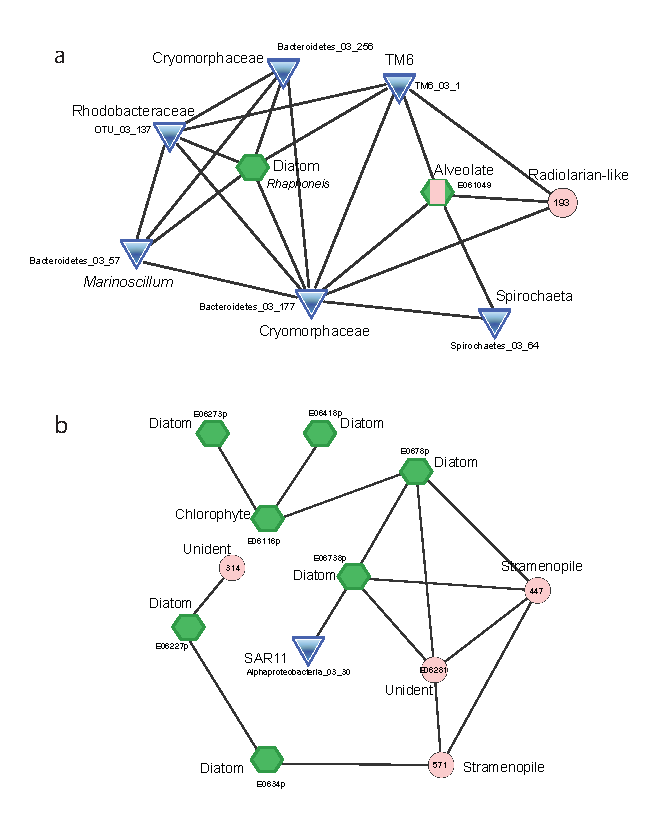
\includegraphics[width=0.9\textwidth]{Chapter_2_MIRADA/Figures/Figure_5_PAL_Ev9Bv6_pooled_50_plusminus90_corr_networkMOD2} 
	\caption[Co-occurrence analysis of combined bacterial and eukaryotic matrices.]{Co-occurrence network analysis of combined bacterial and eukaryotic matrices. Bacteria are indicated by triangles. Lines represent significant Pearson correlations (R>0.9). Pink circles represent microbial eukaryotes that are most likely heterotrophic. Green hexagons represent phototrophs. The pink and green hexagon represents an alveolate of unknown trophic status. (a) A network highlighting Alveolate-Radiolarian interactions, (b) a network focusing on SAR11 and an unknown diatom interaction.} 
	\label{fig:cooccur1} 
\end{figure}

\subsection{Richness and community composition}\label{ssc:richness-and-community-composition}

We detected the highest richness within the bacterial domain (Table \ref{ch1:tab2}, Figure \ref{fig:richness1}a). We observed 234 bacterial OTUs on average with an estimated richness of 520. As with community composition, bacterial richness varied by depth, with 100-m samples having greater observed and estimated diversity (Table \ref{ch1:tab2}, Figure \ref{fig:richness1}a). The winter sample had almost twice the estimated richness (2125) of any summer sample. Over half (51\%) of sequences were classified to the genus level, while an additional 32\% of sequences were identified to the family level. The majority (75 $\pm$ 2\%) of sequences were identified as Proteobacteria, primarily in the Alpha- (36 $\pm$ 3\%) and Gamma- (33 $\pm$ 2\%) subgroups (Figure \ref{fig:ch1:supp1}). Alphaproteobacteria, especially Rhodobacterales, were more important in surface samples, accounting for 43 $\pm$ 2\% of sequences compared to 30 $\pm$ 4\% at 100-m. Inshore surface samples were distinguished by high prevalence of \textit{Roseobacter} (15\% in the north and 6\% in the south). \textit{Candidatus} Pelagibacter (SAR11) was more consistent across surface samples, accounting for 23 $\pm$ 2\% of all sequences. Gammaproteobacteria, primarily SAR86, SAR92, Oceanospirillales, \textit{Balneatrix} and a number of unclassified OTUs, had greater relative abundance in deep samples, accounting for 36 $\pm$ 1\% of sequences. Deltaproteobacteria, especially Desulfobacterales, Nitrospinaceae, and SAR324, were more common at 100-m depth, accounting for 7 $\pm$ 3\% of sequences in deep samples but \textless{}1\% in surface samples. The bulk of the remaining sequences consisted of Flavobacteria, Planctomycetes, and Deferribacteres. Flavobacteria were most abundant in the northern inshore site (28\%). Planctomycetes, especially \textit{Zarvarzinella}, were common at both northern and southern inshore sites (8 $\pm$ 1\%). Deferribacteres were mostly found at 100-m depth (7 $\pm$ 3\%).

\afterpage{
\begin{landscape}
\begin{table}[]
\scriptsize
\centering
\caption[Observed and estimated richness for Bacteria, Archaea, and Eukarya]{Observed and estimated richness for Palmer Station LTER samples using 97\% similarity values for Bacteria and Archaea and 94\% similarity values for Eukarya. Samples for Bacteria and Archaea were pooled unless indicated with a replicate designation after the sample number (e.g. 9.1). Both replicates were used to calculate the eukaryotic diversity estimates. }
\label{ch1:tab2}
\begin{tabular}{@{}lclllllllllll@{}}
    &                                  &           &       & \multicolumn{3}{c}{ARCHAEA}          & \multicolumn{3}{c}{BACTERIA}         & \multicolumn{3}{c}{EUKARYA**}        \\ \midrule
ID  & \multicolumn{1}{l}{Location}     & Depth (m) & Month & No. of Reads & Obs. OTUs & Est. OTUs & No. of Reads & Obs. OTUs & Est. OTUs & No. of Reads & Obs. OTUs & Est. OTUs \\ \midrule
1   & \multirow{2}{*}{Inshore, north}  & 10        & Jan   & -            & -         & -         & 3218         & 126       & 289.4     & 6369         & 211       & 259       \\
1*  &                                  & 10        & Jan   & -            & -         & -         & 3218         & 126       & 289.4     & 4911         & 188       & 229.3     \\
2   & \multirow{2}{*}{Inshore, north}  & 100       & Jan   & 4295         & 21        & 25.7      & 11454        & 513       & 1050.4    & 5568         & 430       & 498       \\
2*  &                                  & 100       & Jan   & 2502         & 20        & 27        & 3218         & 303       & 735.4     & 4911         & 405       & 466.7     \\
3   & \multirow{2}{*}{Offshore, north} & 10        & Jan   & -            & -         & -         & 17676        & 195       & 415       & 4911         & 177       & 194.1     \\
3*  &                                  & 10        & Jan   & -            & -         & -         & 3218         & 103       & 198.8     & 4911         & 176       & 194.5     \\
4   & \multirow{2}{*}{Offshore, north} & 100       & Jan   & 2502         & 21        & 32.3      & 29555        & 350       & 630.3     & 11775        & 313       & 363.5     \\
4*  &                                  & 100       & Jan   & 2502         & 21        & 32.3      & 3218         & 155       & 340.9     & 4911         & 211       & 255.2     \\
5   & \multirow{2}{*}{Offshore, south} & 10        & Jan   & -            & -         & -         & 11845        & 143       & 353.5     & 9078         & 180       & 204.9     \\
5*  &                                  & 10        & Jan   & -            & -         & -         & 3218         & 93        & 176.7     & 4911         & 147       & 169.9     \\
6   & \multirow{2}{*}{Offshore, south} & 100       & Jan   & 9724         & 34        & 45.4      & 21306        & 585       & 1678.4    & 5996         & 407       & 472.6     \\
6*  &                                  & 100       & Jan   & 2502         & 24        & 25.9      & 3218         & 260       & 819.4     & 4911         & 375       & 440.8     \\
7   & \multirow{2}{*}{Inshore, south}  & 10        & Jan   & -            & -         & -         & 4869         & 146       & 303.4     & 7623         & 145       & 162.8     \\
7*  &                                  & 10        & Jan   & -            & -         & -         & 3218         & 120       & 256.8     & 4911         & 125       & 136.4     \\
8   & \multirow{2}{*}{Inshore, south}  & 100       & Jan   & -            & -         & -         & 37524        & 546       & 1551.5    & 11500        & 387       & 431.4     \\
8*  &                                  & 100       & Jan   & -            & -         & -         & 3218         & 206       & 493.9     & 4911         & 285       & 323.3     \\
9.1 & \multirow{2}{*}{Inshore, north}  & 10        & July  & 11941        & 21        & 25.9      & -            & -         & -         & -            & -         & -         \\
9.2 &                                  & 10        & July  & 16026        & 24        & 45.3      & -            & -         & -         & -            & -         & -         \\
9   & Inshore, north                   & 10        & July  & -            & -         & -         & 18410        & 645       & 3474.8    & -            & -         & -         \\
9*  &                                  & 10        & July  & 2502         & 12        & 12.2      & 3218         & 273       & 775.2     & -            & -         & -         \\ \midrule
    &                                  &           &       &              &           &           &              &           &           &              &           &           \\
\multicolumn{3}{l}{*Randomly resampled data.}      &       &              &           &           &              &           &           &              &           &           \\
\multicolumn{3}{l}{**Metazoan reads removed.}      &       &              &           &           &              &           &           &              &           &          
\end{tabular}
\end{table}
\end{landscape}
}


Eukaryotic rRNA gene V9 hypervariable-region sequencing yielded an overall average of 260 observed and 300 estimated OTUs. We did not sequence eukaryotic winter samples so we are unable to contrast seasonal richness patterns in eukaryotes; however, we can say that overall, deeper samples were significantly richer than surface samples. More importantly, we detected increased eukaryotic richness in surface (10 m) and deep (100 m) inshore northern stations as compared to southern ones, but offshore northern and southern stations revealed either no difference or increased richness at depth in the south. Surprisingly, dinoflagellate-related OTUs that constituted the largest eukaryotic OTU class type in our dataset (Figure \ref{fig:ch1:supp2}) did not show depth patterns that were consistent with our expectation that photoautotrophs dominate the euphotic zone and heterotrophs deeper waters, nor did high-performance liquid chromatography-derived pigment data suggest that a disproportionate fraction of the phototrophic community was composed of dinoflagellates. Cryptophytes and diatoms, also among the numerically dominant phototrophs, did not show surface and depth contrasts that might be anticipated of strict phototrophy. This is in contrast to groups like haptophytes which showed increased amplicon read numbers at 10-m vs.~100-m depths. Within 10-m samples, we observed greater relative abundances of cryptophytes at inshore sites while offshore sites were dominated by dinoflagellates and diatoms (Figure \ref{fig:ch1:supp2}). Archaea had the lowest richness of the three domains, with an average of 22 observed and 33 estimated OTUs (Table \ref{ch1:tab2}). Marine Group I Crenarchaeota (MG1: Thaumarchaeota) and Marine Groups II and III (MG2, MG3) Euryarchaeota dominated our samples accompanied by a number of less abundant Thermoplasmatales, Halobacteriales, and Methanosarcinales. MG3 was significantly more abundant ($p<0.05$) in our summer northern inshore and southern offshore samples (8\% relative abundance vs.~0.5\% for all other samples). The winter assemblage differed from summer assemblages with a higher abundance of Thaumarchaeota (80\%) and a lower abundance of MG2 (19\%).



\section{Discussion}\label{sc:discussion}

\subsection{Seasonal, vertical and spatial variation in phytoplankton-heterotroph coupling}\label{ssc:seasonal}

We observed significant differences in microbial community structure (and apparent differences in archaeal abundance) based on depth (10-m and 100-m) (bacteria and eukaryotes), proximity to shore (eukaryotes) and between winter and summer seasons (bacteria and archaea). Depth-based differences were consistent with previous reports of strong vertical stratification in community composition in other environments \citep{dk05,bpbsblfd09}. Results from CCA showed that bacterial and eukaryotic community composition correlated with salinity and silicate for bacteria and temperature and oxygen for eukaryotes: all factors that are influenced by water column vertical stratification. In this context, the similarity between our 10-m surface winter sample and our 100-m summer samples is not surprising. This similarity reflects the origin of the summertime, minimally-modified remnant ``Winter Water'' below the seasonal thermocline \citep{msisv08,dsvse12}. During the Antarctic winter, the water column is divided into two main water masses: warm, nutrient-rich Circumpolar Deep Water (CDW) overlaid by cold, relatively fresh Antarctic Surface Water (AASW) \citep{cmmkpbs07,msisv08}. The AASW results from convective mixing and cooling in winter and can extend to several hundred meters in depth. In the spring, increasing surface temperatures and meltwater from sea ice and glaciers result in water column stratification and the isolation of a deep remnant of the cold, now relatively saline AASW. This cold remnant with a core at about 100 meters is traditionally known as Winter Water (WW) \citep{m34}. Previous findings suggested that WW 100-m communities in summer and winter surface microbial communities might share some features, including more abundant archaea \citep{mtmwjd98,Church2003-oj}. Furthermore, in a comparison of clone libraries generated from winter and summer surface water samples, \citet{grwddecm12} found increased abundance of genes related to chemolithoautotrophy, typically found in deeper marine habitats, during the Antarctic winter. Our results demonstrate that seasonal patterns in WAP water column structure are reflected in bacterial and archaeal community composition.

Several lines of evidence suggest that the mechanism driving the observed succession of microbial community structure from winter to summer is enrichment by organic matter generated by photoautotrophs. Order of magnitude increases in bacterial production rates \citep{dsvse12} must be accompanied by increased resources. The summer bacterial community is characterized by many sequences indicating heterotrophic capabilities \citep{grwddecm12}. Microautoradiography-FISH determinations showed that the most abundant OTUs utilized amino acids and dissolved proteins \citep{straza2010abundance}. A summer bacterial community from the WAP demonstrated reduced diversity in response to experimental glucose enrichment, consistent with our field observations \citep{dmegm11}. In contrast, a summertime sample from the Mediterranean Sea grown over five generations (15 days) in continuous culture in the presence of a complex substrate derived from a phytoplankton culture exhibited increased diversity relative to an unamended control \citep{lckbo13}. The samples and experimental conditions differed between these experiments, preventing simple conclusions about relationships between organic enrichment and diversity.

In the present study, we did not find a significant correlation between phytoplankton biomass and bacterial community composition within summer 10-m samples, although CCA analyses showed silicate to be a significant factor influencing bacterial community structure. The LTER study grid encompasses an inshore-offshore gradient with average (1993-2013) phytoplankton biomass ranging from 4 mg chl \textit{a} m$^{-3}$ on the coast to 0.3 mg chl \textit{a} m$^{-3}$ over the continental slope (\url{http://pal.lternet.edu/data};  \citealt{gvf05,sdv96,sbbs98,sbv98}). We observed high phytoplankton biomass (chl \textit{a}) at the inshore stations in the present study. Despite marked differences in chlorophyll and eukaryotic community composition, unlike eukaryotic communities, bacterial community composition between inshore and offshore sites was only significantly different at the 90\%, but not at the 95\% confidence level based on our ANOSIM analyses. While eukaryotic communities were much less similar to each other overall than bacterial communities, caution should be applied in interpreting absolute magnitudes of the similarity values between abundance-based data (bacteria) and presence/absence (eukaryotes) data. We suggest that none of the surface bacterial communities were carbon-limited in summer but that the relative differences in phytoplankton biomass between sites may have in some way influenced bacterial community composition.

\subsection{Community composition across three domains}\label{ssc:community}

Most studies of bacterial diversity in Antarctic waters have used culture-dependent or community fingerprinting techniques. For example, significant inter-seasonal variation in bacterial community composition was found using DGGE \citep{mpmtbwd98,mg07}. A few studies have used clone libraries to investigate bacterial diversity, finding high diversity within the Gammaproteobacteria and Cytophaga-Flavobacteria-Bacteroidetes (CFB) divisions \citep{ggdsad06,Piquet2011-ot}. More recently, studies have adopted next-generation sequencing approaches to contrast sub-Antarctic and Antarctic bacterial community richness, structure and biogeography \citep{Ghiglione2012-qm, wlwdbhamrrc13, wvrlc13}.

Alphaproteobacteria, Gammaproteobacteria, and Bacteroidetes dominated the bacterial communities we sampled (c.f. \citet{ggdsad06, pcrbslth07, Piquet2011-ot,Ghiglione2012-qm, wlwdbhamrrc13, wvrlc13}. We identified abundant amplicons from several ``ubiquitous'' clusters such as SAR11, SAR86, and SAR324 \citep{pph05}, but also noted the absence of cyanobacteria such as \textit{Prochlorococcus} and \textit{Synechococcus} that are typically absent or rare in bacterial communities in the Antarctic Zone \citep{wlwdbhamrrc13,wywabdlc13}. In addition to the ubiquitous and dominant SAR11, \textit{Roseobacter} was another significant alphaproteobacterium that was likely associating with phytoplankton at shallow depths \citep{Ghiglione2012-qm,wlwdbhamrrc13,wywabdlc13}.

Despite a growing body of knowledge, linking microbial community composition to function remains a significant challenge. However, the contrasts we observed among the abundances of different taxa are suggestive of coupling between primary productivity and bacterial/archaeal presence and community composition. Although overall community composition did not vary significantly among surface samples, a few clades displayed marked differences in relative abundance between sites, indicating different ecological niches at different sampling locations. For example, Planctomycetes, especially \textit{Zarvarzinella}, were more abundant at near-shore sites where algal biomass was highest, in contrast with previous studies wherein Planctomycetes were detected in low abundance in the Southern Ocean \citep{wywabdlc13}. Culture-dependent and -independent techniques have shown that the CFB division is particularly prominent in situations with high DOC availability, e.g. in sea ice \citep{bkjwah03} or during phytoplankton blooms \citep{Glockner1999-yc,Abell2005-vh} perhaps due to superior competitive exploitation of algal-derived carbon \citep{pfgwwa11}. Positive associations between diatoms and Rhodobacteraceae, Cryomorphaceae, and SAR11 respectively in our study also suggest coupling between heterotrophs and photoautotrophs. The significantly increased relative abundance of some proteobacterial clusters (e.g.~Desulfobacterales, Nitrospinaceae, SAR324) in our 100-m samples could indicate that chemolithotrophy is relatively important deeper in the water column \citep{grwddecm12} in the summer. This is consistent with a previous report of Desulfobacterales in winter samples in the Antarctic Peninsula \citep{Ghiglione2012-qm} and SAR324's inferred role in chemautotrophy in the cold, dark ocean \citep{smpswlrpmgsdhs11}. Similarly, archaeal abundance was apparently very low in summer surface waters. These bacterial and archaeal distribution patterns may reflect inability of chemolithotrophs to compete successfully under summer conditions.

A notable aspect of our study was our use of amplicon pyrosequencing to assess the diversity of all three microbial domains, including eukaryotes. Our study detected similar magnitude and trends in increased bacterial richness in winter versus summer as reported previously \citep{Ghiglione2012-qm}, but also added insights into archaeal and eukaryotic richness with depth and location relative to the shoreline. Namely, archaea showed opposite trends to bacteria with decreased richness in our resampled datasets in the winter versus summer with overall numbers of OTUs an order of magnitude less than bacteria and eukaryotes. Like bacteria, eukaryotes also displayed increased richness at depth while archaeal richness at different depths was difficult to ascertain given our inability to detect archaea in summer surface samples.

Previous studies of WAP eukaryotic diversity have relied primarily on pigment data and microscopy \citep{rvz02, rjbf02, gvfsrq03, gvkf03, acccg10} or only considered richness \citep{amdh09}. Large diatoms and cryptomonads generally account for the bulk of phytoplankton biomass, while unidentified photosynthetic flagellates are numerically dominant \citep{vhh93, rjbf02, gvkf03, acccg10}. \citet{gvkf03} observed strong inshore-to-offshore gradients in biomass and community composition and attributed differences between northern and southern inshore blooms (cryptomonads in the north versus diatoms in the south) to differential timing of sea ice retreat. Diatom assemblages are highly variable from year to year \citep{acccg10}, although several genera including \textit{Corethron}, \textit{Chaetoceros}, \textit{Fragilariopsis}, \textit{Odontella}, and \textit{Nitzschia} are common \citep{gvfsrq03,acccg10}, and often co-occur with \textit{Phaeocystis antarctica} \citep{rjbf02, gvkf03}. Cryptophytes were more prevalent in the northern surface waters, but dinoflagellates were the most abundant OTU in our study. The prevalence of dinoflagellates was not consistent with our pigment data or microscopic observations. One likely explanation for over-representation of dinoflagellate-related OTUs may be that dinoflagellates are known to possess many copies of their rRNA genes (\textgreater{}12,000 for dinoflagellates such as \textit{Akashiwo sanguinea}; \citealt{zmnmv05}), while picoeukaryotes may have four orders of magnitude fewer. Another more speculative explanation is that perhaps the dinoflagellate signals detected in large quantities in our study are the result of these cells engaging in kleptoplasty (chloroplast theft from other phototrophs) \citep{gmdc07} allowing them to serve as mixotrophs as needed. This may also help explain why we failed to see dinoflagellate-specific pigment signatures in our HPLC data. Another possible explanation is that the detected dinoflagellate signal derives from heterotrophic and not phototrophic dinoflagellates. Results of our network analyses pointed to Group I alveolates known to include parasitic and therefore heterotrophic clades as possible contributors to eukaryotic niche diversity as a whole. Furthermore, diatom and cryptophyte abundance did not vary significantly with depth, suggesting possible alternative survival strategies such as mixotrophy or heterotrophy \citep{bacccgps00,tsrg06} or possible persistence of environmental DNA \citep{cvcl12,cvl12}.

\subsection{Microbial Diversity, Resilience, and Climate Change}\label{microbial-diversity-resilience-and-climate-change}

\citet{cltcl11} conducted a similar, 3-domain pyrosequencing study in the Amundsen Gulf, Canadian Arctic over the 2003-2010 period of rapid warming and sea ice loss. They observed significant changes in community composition within the bacterial, archaeal and eukaryotic domains over time, and reductions in overall bacterial diversity when samples were pooled into pre- and post-2007 groups. The Palmer LTER study region encompasses a strong climatic gradient running roughly north to south along the Antarctic Peninsula \citep{msisv08,smsi08}. Changes have been more dramatic in the northern part of the region, with greater atmospheric and ocean warming \citep{mk05} and larger reductions in sea ice cover. In response the region has experienced reductions in the populations of ice-dependent species such as Adèlie penguins \citep{dcddghmmmms12}, Antarctic krill \citep{aspr04} and large-celled phytoplankton \citep{mddfmss09} over the past few decades. Thus the WAP presents north and south regions at different stages of climate change, sea ice reduction and ecosystem transformation. It is intriguing that despite well-documented latitudinal trends in phytoplankton and higher trophic levels, we only observed significant differences in microbial richness among eukaryotic microbes and not their bacterial and archaeal counterparts. These differences in eukaryotic richness were not consistent between inshore and offshore sites so we assume that they are not merely the effect of diversity increases due to environmental DNA from surface waters. Beta-diversity patterns between northern and southern stations were less obvious except perhaps for northern inshore eukaryotic communities. These observations relate to ongoing questions about microbial biogeography and community resilience.

The similarity observed between northern and southern assemblages may reflect the timing of sampling. We found that the oceanographic conditions at our sampling sites were quite similar at this time (Table \ref{ch1:tab1}). Many WAP latitudinal trends (i.e.~temperature and sea ice duration and extent) are most apparent during autumn, winter, and spring \citep{dcddghmmmms12}. Properties such as sea ice extent or primary production may or may not reflect gradients or longer-term trends in any single year.

Microbial communities can be similar at kilometer distances but dissimilar tens to hundreds of km apart, supporting the idea of coherent community patches in the open sea \citep{hscf06,mncawa12}. Surface currents in the WAP are \textasciitilde{} \SIrange{0.1}{1}{\meter \per\second} \citep{sa09}, giving an advective timescale between the northern and southern stations of 5-10 days. Bacterial assemblages should have ample time for turnover during transit, so latitudinal similarity over this distance due simply to physical mixing is unlikely \citep{wvrlc13}.

Microbial community resilience may also contribute to the observed lack of variation between northern and southern sites overall. Microbial community composition can be sensitive to disturbances in temperature and carbon enrichment among other factors \citep{am08}. However, fast growth rates, metabolic flexibility, and rapid evolution could increase the stability of microbial community composition and facilitate return to a pre-disturbance state. Microbial communities might vary between the north and south during the winter and spring when greater environmental differences are observed, but then quickly reach a common summer community composition. In contrast, larger, longer-lived organisms integrate the effects of change over years (krill) to decades (penguins, seals).

\section{Conclusions}\label{conclusions}

Analysis of microbial eukaryotic, bacterial and archaeal communities from four sites separated by 200 (cross-shelf) and 400 km (alongshelf) along the WAP revealed relatively low spatial variability in microbial community composition. Community composition responded more to the environmental variability represented by 10-m and 100-m depths than to more subtle differences in production and climate forcing between different sites. Northern versus southern patterns in richness were only represented in inshore microbial eukaryotic communities. Furthermore, we found that bacterial and archaeal assemblages in 100-m summer samples were similar to winter surface (10-m) communities reflecting established seasonal patterns in water column stratification and turnover. While we can begin to speculate on relative differences in community function based on SSU rRNA gene amplicon sequencing, further efforts are needed to examine the abundance and expression of functional genes in order to find the connections between microbial communities and ecosystem function in this fragile and rapidly changing region.

